\documentclass[a4paper]{article}
\usepackage{fullpage}
\usepackage{amsmath}
\usepackage{amssymb}
\usepackage{breqn}
\usepackage{sectsty}
\usepackage{graphicx}
\usepackage{svg}
\usepackage{xcolor}
\usepackage{esint}
\usepackage{pdfpages}
\usepackage{fancyhdr}
\usepackage{chngcntr}
\usepackage{pagecolor}
\usepackage{caption}
\usepackage{subcaption}
\usepackage{physics}
\usepackage{float}
\counterwithin*{equation}{section}
\counterwithin*{equation}{subsection}
\renewcommand{\thesubsection}{\thesection.\alph{subsection}}
\renewcommand{\thesubsubsection}{\Roman{subsubsection}}
\newcommand{\horln}{\vspace{-6mm}\begin{flushleft}\mbox{}\hrulefill\mbox{}
	\end{flushleft}\vspace{-6mm}}
\newcommand\eq{\addtocounter{equation}{1}\tag{\theequation}}
\sectionfont{\huge}
\subsubsectionfont{\small}
\setlength{\parindent}{0cm}
\usepackage[citestyle=ieee]{biblatex}
\title{PHYS4123 GR Assignment 1}
\author{SID: 480344342}
\begin{document}
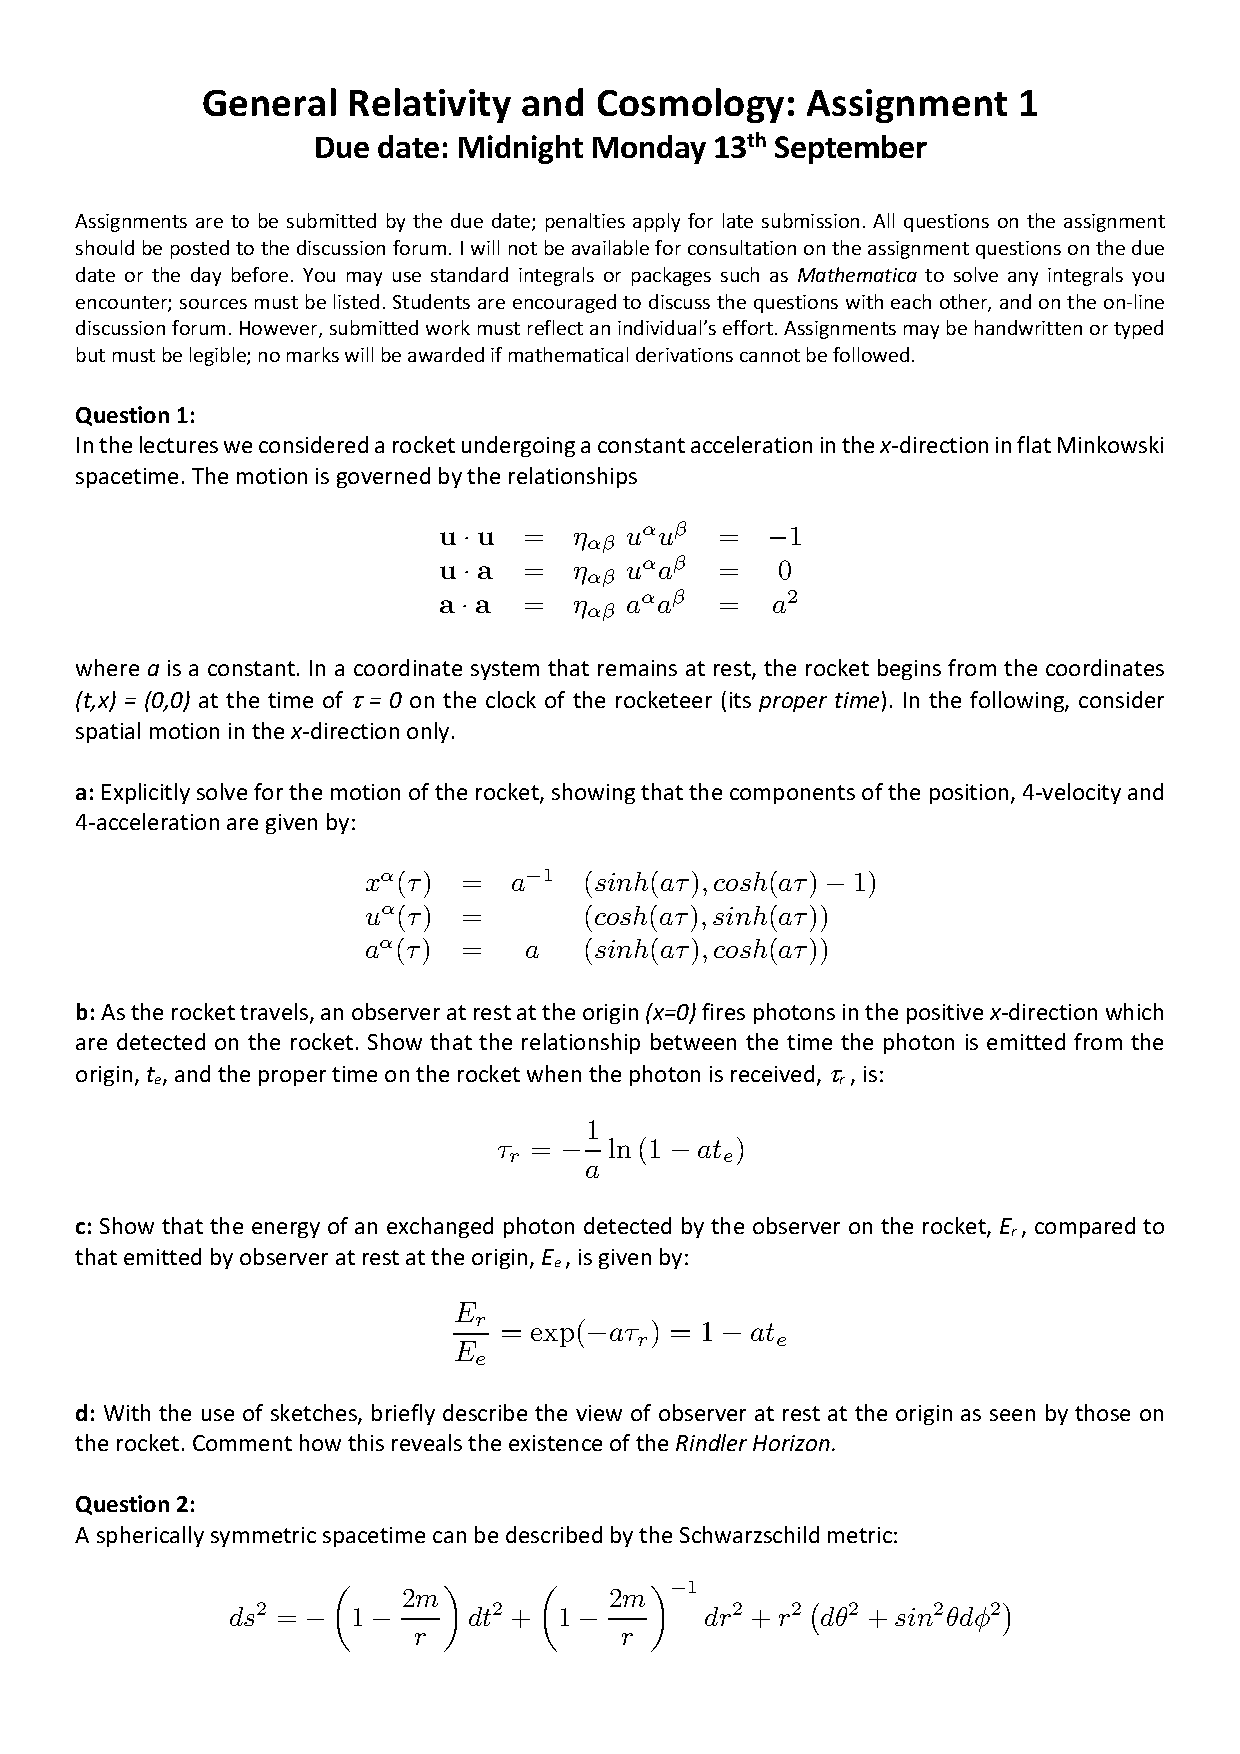
\includepdf[pages=-]{Figures/Questions}
\maketitle
\horln

\setcounter{page}{1}

%  *  ██████   ██
%  * ██    ██ ███
%  * ██    ██  ██
%  * ██ ▄▄ ██  ██
%  *  ██████   ██
%  *     ▀▀

\section{}
\subsection{}
Given:
\begin{align*}-1 &= \eta_{\alpha \beta} u^\alpha u^\beta\\
0 &= \eta_{\alpha \beta} u^\alpha a^\beta \\
a^2 &= \eta_{\alpha \beta} a^\alpha a^\beta
\end{align*}
Assuming spatial motion only occurs in $x^1$ gives:
\begin{align*}
-1 &= -u^0u^0 + u^1u^1\\
0 &= -u_0a_0 + u_1 a_1\\
a^2 &= -a^0a^0 + a^1a^1
\end{align*}
Then:
\begin{align*}
u^0u^0 &= u^1u^1 + 1 \eq \label{eq:1}\\
a_0 &= \frac{u_1}{u_0} a_1 \eq \label{eq:2}\\
a^1a^1 &= a^0a^0 + a^2 \eq \label{eq:3}
\end{align*}

Substituting \eqref{eq:2} into \eqref{eq:3}:
\begin{align*}
a^1a^1 &= a^2 \frac{1}{1-u^1u^1/u^0u^0}\\
a^0a^0 &= a^2 \frac{1}{u^0u^0/u^1u^1 - 1}
\end{align*}

Then using \eqref{eq:1}:
\begin{align*}
a^1a^1 &= a^2 (1 + u^1 u^1) = \left(\frac{du^1}{d\tau}\right)^2\\
a^0a^0 &=  a^2 (u^0 u^0 - 1) =  \left(\frac{du^0}{d\tau}\right)^2
\end{align*}

Integrating:
\begin{align*}
\tau &= \pm \int \frac{1}{\abs{a}\sqrt{1 + u^1 u^1}} du^1 = \pm \frac{1}{\abs{a}}\sinh^{-1}(u^1) + A\\
\tau &= \pm \int \frac{1}{\abs{a}\sqrt{u^0 u^0 - 1}} du^1 = \pm \frac{1}{\abs{a}}\cosh^{-1}(u^0) + B
\end{align*}
Assuming $u^0 > 0$. Since the rocket begins at rest, $(u^0, u^1) = (1, 0)$ at $\tau = 0$ and$C = 0$ and $B = 0$. Also, letting $\mp \abs{a} = a$ (such that the sign of $a$ is the direction of $a^1$):
\begin{align*}
(u^0, u^1) &= (\cosh(a \tau), \sinh(a\tau))
\end{align*}
Differentiating gives:
\begin{align*}
	(a^0, a^1) &= a(\sinh(a \tau), \cosh(a\tau))
\end{align*}
Whereas integrating gives:
\begin{align*}
	(x^0, x^1) &= \frac{1}{a}(\sinh(a \tau) + C, \cosh(a\tau) + D)
\end{align*}
Where the initial conditions $(x^0, x^1) = (0, 0)$ at $\tau = 0$ constrain $C = 0$ and $D = -1$.



\subsection{}
A shown in figure~\ref{fig:1}, a photon launched at $t_e$ by a stationary observer will intersect with the world line of the rocket, if it is correctly aimed. 
The photon's world line is a straight line with gradient $1$ (a speed of $c$) intersecting $x=0$ at $t_e$: $t -  t_e = x$.
The rockets world line is the curve $(x, t) = x^\alpha(\tau)$, derived in part $a$.
The intersection of these two world lines occurs when:
\begin{align*}
	\frac{1}{a}\cosh(a\tau) - \frac{1}{a} &= \frac{1}{a} \sinh(a\tau) - t_e\\
	\implies 1-at_e &= \cosh(a\tau) - \sinh(a\tau) \\
	&= e^{-a \tau}\\
	\implies -a \tau &= \ln(1-at_e)\\
	\implies \tau &= -\frac{1}{a} \ln(1-at_e)\\
\end{align*}






%  *  ██████  ██████▄
%  * ██    ██      ██
%  * ██    ██ ▄█████▀
%  * ██ ▄▄ ██ ██
%  *  ██████  ███████
%  *     ▀▀

\section{}
\subsection{}
% Since the proper time is:
% \begin{align*}
% 	\tau = \int_0^1 -d\sigma ds,
% \end{align*}
% for some parameterisation by $\sigma$ of a path is spacetime, 
The Lagrangian equivalent $K$ for the Schwarzschild metric is:
\begin{align*}
	K &= g_{\alpha \beta} \frac{dx^\alpha}{d\tau} \frac{dx^\beta}{d\tau}\\
	&=	-\left( 1- \frac{2m}{r}\right) \left( \frac{dt}{d\tau} \right)^2 + \left( 1- \frac{2m}{r}\right)^{-1} \left( \frac{dr}{d\tau} \right)^2    + r^2 \left( \frac{d\theta}{d\tau} \right)^2  + r^2 \sin^2(\theta) \left( \frac{d\phi}{d\tau} \right)^2  . 
\end{align*}
Then:
\begin{align*}
\frac{\partial K}{\partial \left(dx^\alpha / d\tau \right)} &= 2\left[-\left( 1- \frac{2m}{r}\right) \frac{dt}{d\tau} , \left( 1- \frac{2m}{r}\right)^{-1} \frac{dr}{d\tau} , r^2 \frac{d\theta}{d\tau} , r^2 \sin^2(\theta) \frac{d\phi}{d\tau} \right], \\
%\implies \frac{d}{d\tau} \frac{\partial K}{\partial \left(dx^\alpha / d\tau \right)}  &= 2 \left[-\left( 1- \frac{2m}{r}\right) \frac{d^2t}{d\tau^2} , \left( 1- \frac{2m}{r}\right)^{-1} \frac{d^2r}{d\tau^2} , r^2 \frac{d^2\theta}{d\tau^2} , r^2 \sin^2(\theta) \frac{d^2\phi}{d\tau^2} \right] \\
\intertext{and:}
\frac{\partial K}{\partial x^\alpha} &= 2\left[0, \frac{1}{2}\frac{\partial K}{\partial r}, r^2 \sin(\theta)\cos(\theta) \left( \frac{d\phi}{d\tau} \right)^2, 0 \right],
\end{align*}
where:
\begin{align*}
	\frac{1}{2}\frac{\partial K}{\partial r} &= -\frac{m}{r^2} \left(\frac{dt}{d\tau} \right)^2 - \frac{m}{(r-2m)^2}  \left(\frac{dr}{d\tau} \right)^2 + r  \left(\frac{d\theta}{d\tau} \right)^2  + r\sin^2(\theta)  \left(\frac{d\phi}{d\tau} \right)^2.
\end{align*}
Using the Euler-Lagrange equation:
\begin{align*}
\frac{d}{d\tau} \frac{\partial K}{\partial(dx^\alpha / d\tau)}  = \frac{\partial K}{\partial x^\alpha},
\end{align*}
gives:
\begin{align*}
	\frac{d}{d\tau} \left[ \left(1-\frac{2m}{r}\right) \frac{dt}{d\tau} \right] &= 0\\
	\frac{d}{d\tau} \left[ \left( 1- \frac{2m}{r}\right)^{-1} \frac{dr}{d\tau} \right] &=  -\frac{m}{r^2} \left(\frac{dt}{d\tau} \right)^2 - \frac{m}{(r-2m)^2}  \left(\frac{dr}{d\tau} \right)^2 + r  \left(\frac{d\theta}{d\tau} \right)^2  + r\sin^2(\theta)  \left(\frac{d\phi}{d\tau} \right)^2\\
	\frac{d}{d\tau} \left[ r^2 \frac{d\theta}{d\tau}  \right]  &= r^2 \sin(\theta)\cos(\theta) \left( \frac{d\phi}{d\tau} \right)^2 \\
	\frac{d}{d\tau} \left[r^2 sin^2(\theta) \frac{d\phi}{d\tau} \right] &= 0
\end{align*}



\subsection{}
Expanding and rearranging the equations of motion above:
\begin{align*}
	\left(1-\frac{2m}{r}\right) \frac{d^2 t}{d\tau^2}  + \frac{dt}{d\tau} \frac{2m}{r^2} \frac{dr}{d\tau}  &= 0\\
	\frac{d^2r}{d\tau^2} \frac{r}{r-2m} - \left(\frac{dr}{dt}\right)^2 \frac{2m}{(r-2m)^2}&=   -\frac{m}{r^2} \left(\frac{dt}{d\tau} \right)^2 - \frac{m}{(r-2m)^2}  \left(\frac{dr}{d\tau} \right)^2 + r  \left(\frac{d\theta}{d\tau} \right)^2  + r\sin^2(\theta)  \left(\frac{d\phi}{d\tau} \right)^2 \\
	r^2 \frac{d^2\theta}{d\tau^2} + 2r \frac{dr}{d\tau} \frac{d\theta}{d\tau}  &= r^2 \sin(\theta)\cos(\theta) \left( \frac{d\phi}{d\tau} \right)^2 \\
	r^2 \sin^2(\theta) \frac{d^2\phi}{d\tau^2} + 2r \sin^2(\theta) \frac{d\phi}{d\theta} + 2r^2 \cos(\theta) \sin(\theta) \frac{d\theta}{d\tau} &= 0
\end{align*}
Then:
\begin{align*}
	\frac{d^2 t}{d\tau^2} &= - \frac{2m}{r^2} \left(1-\frac{2m}{r}\right)^{-1} \frac{dt}{d\tau}  \frac{dr}{d\tau}\\
	\frac{d^2r}{d\tau^2} &=   -\frac{m}{r^2} \left(1-\frac{2m}{r}\right) \left(\frac{dt}{d\tau} \right)^2 + \frac{m}{r^2\left(1-\frac{2m}{r}\right)^2}  \left(\frac{dr}{d\tau} \right)^2 + (r - 2m)  \left(\frac{d\theta}{d\tau} \right)^2  + (r - 2m)\sin^2(\theta)  \left(\frac{d\phi}{d\tau} \right)^2\\
	\frac{d^2\theta}{d\tau^2}  &= \sin(\theta)\cos(\theta) \left( \frac{d\phi}{d\tau} \right)^2 - \frac{2}{r} \frac{dr}{d\tau} \frac{d\theta}{d\tau} \\
	 \frac{d^2\phi}{d\tau^2} &= - \frac{2}{r}  \frac{d\phi}{d\theta} - 2 \frac{\cos(\theta)}{ \sin(\theta)} \frac{d\theta}{d\tau}
\end{align*}
The general geodesic equation is:
\begin{align*}
\frac{d^2 x^\alpha}{d\tau^2} &= -\Gamma^\alpha_{\beta \gamma} \frac{dx^\beta}{d\tau}\frac{dx^\gamma}{d\tau}
\end{align*}
Comparing the the rearranged equations of motion above, this gives:
\begin{align*}
justwritethemout
\end{align*}



\subsection{}
Since the metric is diagonal ($g^{\alpha \beta} = 0$ when $\alpha \ne \beta$), the relationship between the metric and the Christoffel symbols can be simplified to:
$$\Gamma^\alpha_{\beta \gamma} = \frac{1}{2} g^{\alpha \alpha}(g_{\beta \beta , \gamma} + g_{\gamma \gamma , \beta} - g_{\beta \gamma , \alpha}), $$
since all other terms are zero.

.............justworkthroughthem.............

% Then by the Euler-Lagrange equation (equating the two above expressions):
% \begin{align*}
% 	e &= \left(1-\frac{2m}{r}\right)\frac{d t}{d\tau}\\
% 	l &= r^2 \sin^2(\theta) \frac{d\phi}{d\tau}
% \end{align*}
% where $e$ and $l$ are constant.


% \begin{figure}[H]
%    { \centering
%         \includesvg[width=0.98\textwidth]{Figures/OtherMetals.svg}
%         \caption{\textbf{Valid excitation angles for SPP excitation by four-wave mixing at various metal-dielectric interfaces.} The valid angles depend very little on the type of metal used in the interface. This is especially true when both of the angles are not glancing (not close to $90^\circ$), and is because the wavevector of the SPP does not depend strongly on the relative permittivity of the metal ($k'_i = \frac{\omega'_i}{c} \sqrt{\varepsilon(\omega'_i)}/\sqrt{\varepsilon(\omega'_i)+1}$), where the fraction is close to $1$ since $\varepsilon \gg 1$ (and frequencies do not change with refractive index or relative permittivity).}
%     \label{fig:2}}
% \subsubsection{}
%     {\centering
%         \includesvg[width=0.98\textwidth]{Figures/Au_H20.svg}
%         \caption{\textbf{Valid angles for SPP excitation at an interface between water and gold.} Comparing to Fig. 1, the valid angles have changed significantly, particularly at glancing angles. This is because the real part of the wavevector of the SPP (e.g. $\pm\Re(k'_1) = 2k_1 \sin(\theta_1) - k_2 \sin(\theta_2)$) depends \textit{linearly} on the index of the dielectric ($k = k_0 n$). Comparing to Fig. 2, the index of the dielectric (which strongly changes $\Re(k'_i)$) therefore has a much stronger effect on the valid angles than the $\varepsilon$ of the metal (which weakly changes $k'_i$).}
%     \label{fig:3}}
% \end{figure}

% \includepdf[pages=-]{Plasmonics.pdf}

\end{document}
